%%%% Paramétrage du cours %%%%
\def\xxactivite{Cours}

\fichefalse \proftrue \tdfalse \courstrue

\def\xxnumchapitre{Chapitre 2 \vspace{.2cm}}
\def\xxchapitre{\hspace{.12cm} Représentation des nombres en mémoire}

\def\xxcompetences{%
\textsl{%
\textbf{Savoirs et compétences :}\\
\begin{itemize}[label=\ding{112},font=\color{bleuxp}] 
\item Représentation des entiers positifs sur des mots de taille fixe.
\item Représentation des entiers signés sur des mots de taille fixe.
\item Entiers multi-précision de Python.
\item Distinction entre nombres réels, décimaux et flottants.
\item Représentation entre nombres réels, décimaux et flottants.
\item Représentation des flottants sur des mots de taille fixe. Notion de mantisse, d'exposant. 
\item Précision des calculs en flottants.
\end{itemize}
}}

\def\xxfigures{
%\includegraphics[width=\linewidth]{matlab}
%\\
%\textit{Modèle du pilote hydraulique avec pilotage interactif.}
}%figues de la page de garde

\input{\repRel/Style/pagegarde_cours_minitoc}
\setlength{\columnseprule}{.1pt}

\vspace{2cm}
\pagestyle{fancy}
\thispagestyle{plain}

%%%%%%%%%%%%%%%%%%%%%%%

\section{Bases de numération}

Le système de numération courant est le système décimal (ou base 10). 
On décompose un entier en dizaines, centaines, milliers, etc. 
L'essentiel est alors qu'il y ait strictement moins de dix éléments dans chaque type de paquet. Ce nombre d'éléments peut être représenté par un chiffre.
On écrit alors tous les chiffres à la suite. À gauche, on place les \textbf{chiffres de poids fort} (\textit{most significant digit}). À droite, les \textbf{chiffres de poids faible}  (\textit{least significant digit}).

Ainsi $2735$ représente deux milliers plus sept centaines plus trois dizaines plus cinq unités.

\begin{defi}{Ecriture d'un nombre dans une base }
De manière générale :%, avec $B=10$ et $n\in\N$,
$$\displaystyle\underline{a_{n}a_{n-1}\ldots a_{1}a_{0}}_{~B} =
\sum_{k=0}^{n}a_{k}B^{k},~ \textrm{ et }~\forall k \in \iif{0;n},~ a_k\in\ii{0;B}.$$ 
On note $B$ la base, $a_k$ le chiffre de rang $k$.
\end{defi}

\begin{exemple}
Décomposition de 247 en base 10 : $247_{(10)} = 2\cdot 10^2 + 4\cdot 10^1 + 7\cdot 10^0$.

Décomposition de $1001_2$ en base 2 : $1001_2 = 1\cdot 2^{11_2} + 0\cdot 2^{10_2} + 0\cdot 2^{1_2} + 1\cdot 2^{0_2} 
= 1\cdot 2^{3_{10}} + 0\cdot 2^{2_{10}} + 0\cdot 2^{1_{10}} + 1\cdot 2^{0_{10}}$.
\end{exemple}



\subsection{Les systèmes de numération}
\subsubsection{Système décimal}
Le système décimal est le système universellement utilisé. C'est la base de référence, ce qui signifie qu'un nombre est de manière implicite écrite en décimal, dès lors qu'il est écrit sans précision de base. 

En python, les chiffres sont \textbf{affichés} par défaut dans le système décimal. 

\subsubsection{Système binaire}

C'est la base de numération couramment utilisée en électronique ou informatique. C'est un système en base 2, l'écriture des nombres est donc composée des caractères de 0 et 1. 

\begin{exemple}~\\

\begin{minipage}[c]{.4\linewidth}
En binaire on compte de la manière suivante : 
\begin{center}
\begin{tabular}{|c|c|}
\hline
Base 10 & Base 2 \\
\hline \hline
0 & 0000 \\ \hline
1 & 0001 \\ \hline
2 & 0010 \\ \hline
3 & 0011 \\ \hline
4 & 0100 \\ \hline
\end{tabular}
\end{center}
\end{minipage} \hfill
\begin{minipage}{.57\linewidth}
\textit{Convertir $\left(11011001\right)_2$ en base 10.}

\textit{Convertir $\left(42\right)_{10}$ en base 2.}
\end{minipage}
\end{exemple}

En Python, il est possible de manipuler des nombres en binaires en utilisant le préfixe \texttt{0b}. Ainsi, \texttt{0b111} est interprété comme l'entier 7. 
Il est aussi possible de convertir des entiers en binaires avec la fonction bin. Le résultat est une chaîne de caractère (\texttt{str}) de la forme \texttt{'0b111'}.

\subsubsection{Système hexadécimal}
Ce système à base 16 est le plus utilisé en électronique numérique car il permet une représentation compacte ce qui, dans les systèmes actuels à grande capacité mémoire, est un avantage non négligeable. 
Ainsi, les chiffres de ce système de numération sont 0, 1, 2, 3, 4, 5, 6, 7, 8, 9, A, B, C, D, E, F.  

\begin{exemple} ~\\
\begin{minipage}[c]{.6\linewidth}
En hexadécimal on compte de la manière suivante : 
\begin{center}
\begin{tabular}{|c|c|c||c|c|c|}
\hline
Base 10 & Base 2 & Base 16 & Base 2 & Base 10 & Base 16 \\
\hline \hline
0 & 0000 & 00 & 10 & 1010 & 0A \\ \hline
1 & 0001& 01 & 11  & 1011 & 0B \\ \hline
2 & 0010& 02 & 12  & 1100 & 0C \\ \hline
3 & 0011& 03 & 13  & 1101 & 0D \\ \hline
4 & 0100& 04 & 14  & 1110 & 0E \\ \hline
5 & 0101& 05 & 15  & 1111 & 0F \\ \hline
6 & 0110& 06 & 16  & 1 0000 & 10\\ \hline
7 & 0111& 07 & 17  & 1 0001 & 11 \\ \hline
8 & 1000& 08 & 18  & 1 0010 & 12 \\ \hline
9 & 1001& 09 & 19  & 1 0011 & 13 \\ \hline
\end{tabular}
\end{center}
\end{minipage}% \hfill
\begin{minipage}[t]{.37\linewidth}
Convertir $\left(BC5 \right)_{16}$ en base 10.

Convertir $192$ en base 16.
\end{minipage}
\end{exemple}


En Python, il est possible de manipuler des nombres en hexadécimal en utilisant le préfixe \texttt{0x}. Ainsi, \texttt{0xA1} est interprété comme l'entier 162. 
Il est aussi possible de convertir des entiers en hexadécimal avec la fonction \texttt{hex}. Le résultat est une chaîne de caractère (\texttt{str}) de la forme \texttt{'0xa1'}.


\subsection{Algorithme de décomposition d'un entier dans une base}
\begin{methode}
La méthode générale pour décomposer un entier $n$ en base $k$ est la suivante :
\begin{itemize}
\item on effectue des divisions euclidiennes successives par k jusqu’à avoir un quotient nul ;
\item on récupère les restes en remontant les calculs.
\end{itemize}
\end{methode}

\begin{lstlisting}
def decomposition(x:int, k:int)->str:
    """Donne la décomposition de l'entier x dans la base k.
    Entrées :
        x(int) : le nombre entier à écrire dans une nouvelle base
        k(int) la base de décomposition
    Sortie :
        le nombre dans la nouvelle base sous forme de chaine de caractères
    """
    n = x
    chaine = ''
    if n==0:
        chaine='0'
    while n > 0:
        r = n % k
        chaine = str(r) + chaine
        n = n // k
    return(chaine)
\end{lstlisting}

\section{Représentation des entiers sur un ordinateur}
\subsection{Cadre}
\begin{defi}{Mot-machine}
En architecture informatique, un mot est une unité de base manipulée par un microprocesseur. On parle aussi de mot machine. La taille d’un mot s’exprime en bits. Elle est souvent utilisée pour classer les microprocesseurs (32 bits, 64 bits, etc.).
\end{defi}

Sur un ordinateur on travaille sur des mots-machine de 64 bits (8 octets).

Les opérations d’addition et de multiplication d’entiers internes au processeur se font sur 64 bits.
De manière générale, on s’intéressera au fonctionnement sur des ordinateurs travaillant sur des mots de $n$ bits
($n \geq 2$).


Par ailleurs, sur les disques durs, les donées sont stockées sous forme binaire. Ainsi, 
un octet = \SI{8}{bits}, un kilo octet~= \SI{1000}{octet} \textit{etc}.


\subsection{Représentation des entiers}
Les entiers sont directement codés en binaire. Lorsque les mots-machines sont codés sur $n$ bits, il est alors possible de coder des nombres compris entre 0 et $2^n-1$.
\begin{rem}
\begin{itemize}
\item On peut alors observer des dépassements de capacité : si les mots sont codés sur 4 bits, $(1100)_2 + (1000)_2 = (0100)_2$ (et non $(10100)_2$). Dans ce cas, la retenue est perdue. 
\item En Pyton, les entiers ne sont pas codés sur un nombre de bits défini. On est seulement limité par la mémoire de la machine.
\end{itemize}
\end{rem}
\subsection{Représentation des entiers relatifs -- Complément à 2}

Lorsque les mots sont codés sur $n$ bits et qu'on souhaite coder des entiers positifs et négatifs, on pourra coder des nombres compris dans l'intervalle $\llbracket-2^{n-1},2^{n-1}-1\rrbracket$. Les nombres positifs seront codés en binaire comme vu précédemment. 

Les nombres négatifs seront codés selon la méthode du complément à 2. 
\begin{methode}
Si les mots sont codés sur $n$ bits, si on souhaite coder $a<0$, $a$ sera codé comme l'entier naturel $a+2^n$. 
\end{methode}

\begin{exemple} 
\begin{multicols}{2}
Soit un système où les entiers relatifs sont codés sur 3 bits. On peut donc coder des nombres compris dans $\llbracket-4,3\rrbracket$.
\begin{itemize}
\item 2 est codé par $2=(010)_2$;
\item $-2$ est codé par $-2+2^3 = 6 = (110)_2$.
\end{itemize}  
\textit{Remarques :}
\begin{itemize}
\item les nombres négatifs commencent donc par $1$;
\item pour convertir $a=(110)_2$ en base 10 lorsque le codage est sur 3 bits, on a :$a= (110)_2 - 2^3 = 6 - 8 = -2$.
\end{itemize}  
\end{multicols}
\end{exemple}

\section{Représentation des nombres réels}
\subsection{Conversion de la partie fractionnaire des nombres réels}

En notation décimale, les chiffres à gauche de la virgule représentent des entiers, des dizaines, des centaines, etc. et ceux à droite de la virgule, des dizièmes, des centièmes, des millièmes, etc.


\begin{exemple}
$$
3,3125_{ (10)}	=	3\cdot 10^0 + 3\cdot10^{- 1} + 1\cdot10^{- 2} + 2\cdot10^{ -3} + 5\cdot10^{ -4}
$$
\end{exemple}

Par analogie, pour écrire un nombre binaire à virgule, on utilise les puissances négatives de 2.

\begin{exemple}
\begin{eqnarray*}
11,0101_{(2)} &=&	1\cdot 2^{1} + 1\cdot 2^{0} + 0\cdot 2^{-1} + 1\cdot 2^{- 2} + 0\cdot 2^{-3} + 1\cdot 2^{- 4}\\
		 &=&    2   +   1   +    0    +   0,25  +     0     +   0,0625\\
		 &=&   3,3125_{(10)}\\
\end{eqnarray*}
\vspace{-1cm}
\end{exemple}


Le codage de la partie entière (3 dans l’exemple précédent) ne pose pas de problèmes particuliers. Pour la partie fractionnaire (0,3125), il est nécessaire d’adapter la procédure.

\begin{methode}
\textbf{Conversion d'une partie fractionnaire en binaire}

\begin{enumerate}
\item On multiplie la partie fractionnaire par 2. 
\item La partie entière obtenue représente le poids binaire (limité aux seules valeurs 0 ou 1). 
\item La partie fractionnaire restante est à nouveau multipliée par 2.
\item On procède ainsi de suite jusqu’à ce qu’il n’y ait plus de partie fractionnaire ou que le nombre de bits obtenus correspond à la taille du mot mémoire dans lequel on stocke cette partie.
\end{enumerate}
\end{methode}


\begin{exemple}
\textit{Conversion de la partie fractionnaire 0,3125}

\begin{center}
\begin{tabular}{cccccc|c|cc}
\cline{7-7}
0,3125 & x & 2 & = & 0,625 & = & 0 & + & 0,625 \\
0,6250 & x & 2 & = & 1,250 & = & 1 & + & 0,250 \\
0,2500 & x & 2 & = & 0,500 & = & 0 & + & 0,500 \\
0,5000 & x & 2 & = & 1,000 & = & 1 & + & 0,000 \\
\cline{7-7}
\end{tabular}
\end{center}
On considère les parties entières de haut en bas :
$0,3125_{(10)}=0,0101_{(2)}$.
%\begin{center}
%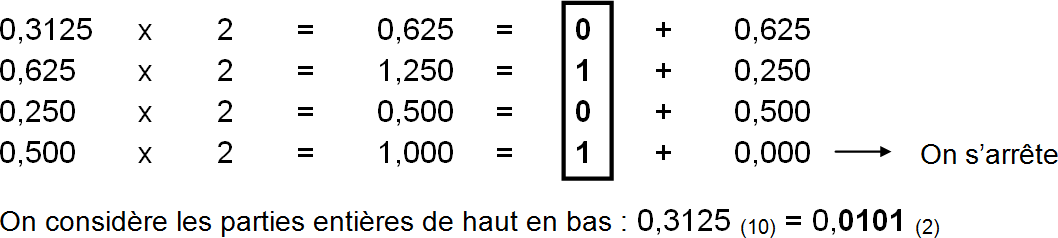
\includegraphics[width=.7\textwidth]{images/reel_0}
%\end{center}
\end{exemple}

%\begin{rem}
%\textbf{Inconvénients}
%
%Savoir coder la partie fractionnaire d’un nombre à virgule ne suffit pas pour coder tous les nombres à virgule en binaire. En effet, la gestion d’une virgule virtuelle par programme n’est pas aisée. De plus, cette méthode ne permet pas de représenter des nombres très grands ou très petits comme le nombre d’Avogadro ($6,02214129.. \cdot  10^{23}$) ou la constante de Planck ($6,62606957 \cdot 10^{- 34}$).
%\end{rem}

\begin{exemple}
\textit{Convertir la partie fractionnaire 0,1}
\end{exemple}

\subsection{Représentation d'un nombre réel en flottant en utilisant la norme IEEE-754}

Pour représenter des réels, nombres pouvant être positifs, nuls, négatifs et non entiers, on utilise la représentation en virgule flottante (\textit{float} en anglais) qui fait correspondre au nombre 3 informations :

$$
-243,25_{(10)} = \underbrace{-}_{1}0,\underbrace{24325}_{2}\cdot10^{\underbrace{3}_{3}}
$$
On appelle alors : 
\begin{enumerate}
\item le signe (positif ou négatif);
\item la mantisse (nombre de chiffres significatifs);
\item l'exposant : puissance à laquelle la base est élevée. 
\end{enumerate}

Sous cette forme normalisée, il suffit de mémoriser le signe, l’exposant et la mantisse pour avoir une représentation du nombre en base 10. Il n’est pas utile de mémoriser le 0 avant la virgule puisque tous les nombres vont commencer par 0. En faisant varier l’exposant, on fait « flotter » la virgule décimale.

Pour représenter un nombre réel dans la machine, il faut préalablement écrire les nombres sous la forme (norme IEEE 754 -- Institute of Electrical and Electronics Engineers) :

\begin{center}
signe 1, mantisse x $2^{\text{exposant}}$.
\end{center}



\begin{exemple}
En binaire, on a $-100110,10101 =  -1,0011010101\times 2^5$ avec $-$ le signe, 0011010101 la mantisse et 5 l'exposant.
\end{exemple}

\begin{minipage}[c]{.4\linewidth}
Le tableau décrit la répartition des bits selon le type de précision : la taille de la mantisse ($m$ bits) donne la précision mais suivant la valeur de l'exposant, la précision sera totalement différente. 

%Ainsi : 
%\begin{itemize}
%\item erreur relative : $2^{-m}$ (poids du dernier bit)
%\item erreur absolue : erreur relative * $2^{\text{exposant}}$
%\end{itemize}
%
%Simple précision :  	$2^{- 23} = 1,192 … * 10^{- 7}$ 
%Double précision :  	$2^{- 52} = 2,220 … * 10^{- 16}$


\end{minipage}\hfill
\begin{minipage}[c]{.59\linewidth}
\begin{center}
\begin{tabular}{| l |c|c|c|}
\hline

& Signe & Exposant & Mantisse \\ \hline
 Simple précision -- 32 bits & 1 & 8 & 23 \\ \hline
 Double précision -- 64 bits & 1 & 11 & 52 \\ \hline
 Précision étendue -- 80 bits & 1 & 15 & 64 \\ \hline
\end{tabular}
\end{center}
\end{minipage}


\begin{methode}
\begin{enumerate}
\item Convertir en binaire les partie entière et fractionnaire du nombre sans tenir compte du signe.
\item Décaler la virgule vers la gauche pour le mettre sous la forme normalisée (IEEE 754).
\item Codage du nombre réel avec les conventions suivantes : 
\begin{itemize}
\item signe = 1 : Nombre négatif 	(Signe = 0 : Nombre positif);
\item le chiffre 1 avant la virgule étant invariant pour la forme normalisée, il n’est pas codé;
\item on utilise un exposant décalé au lieu de l’exposant simple (complément sur octet). Ainsi, on ajoute à l’exposant simple la valeur 127 en simple précision et 1023 en double précision (c’est à dire $2^{n-1}-1$ où $n$ est le nombre de bits de l’exposant);
\item la mantisse est complétée à droite avec des zéros.
\end{itemize}
\end{enumerate}
\end{methode}


\begin{exemple}
On désire représenter le nombre - 243,25 en virgule flottante au format simple précision.

\begin{enumerate}
\item $\quad 243,25_{(10)} =  11110011,01_{(2)}$
\item $\quad 243,25_{(10)} =  1,111001101_{(2)} \times  2^7$ : décalage de 7 bits vers la gauche
\item Exposant décalé : $7 + 127 = 134_{(10)} = 1000\; 0110_{(2)}$ 	sur $n$ = 8 bits
\item $111001101\quad 00000000000000$
\end{enumerate}
\end{exemple}

%\begin{center}
%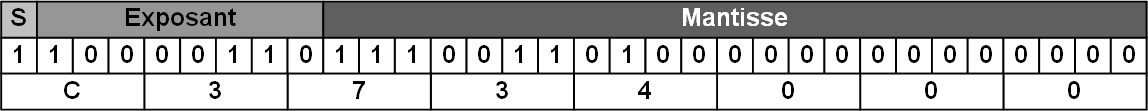
\includegraphics[width=.7\textwidth]{images/reel_2}
%\end{center}

\footnotesize{
\begin{center}
\begin{tabular}{|c|c|c|c|c|c|c|c|c|c|c|c|c|c|c|c|c|c|c|c|c|c|c|c|c|c|c|c|c|c|c|c|}
\hline
S & \multicolumn{8}{c|}{Exposant} & \multicolumn{23}{c|}{Mantisse} \\
\hline
1 & 1 & 0 & 0 & 0 & 0 & 1 & 1 & 0 & 1 & 1 & 1 & 0 & 0 & 1 & 1 & 
0 & 1 & 0 & 0 & 0 & 0 & 0 & 0 & 0 & 0 & 0 & 0 & 0 & 0 & 0 & 0 \\
\hline
\multicolumn{4}{|c|}{C} & \multicolumn{4}{c|}{3} & \multicolumn{4}{c|}{7} & 
\multicolumn{4}{|c|}{3} & \multicolumn{4}{|c|}{4} & \multicolumn{4}{c|}{0} & 
\multicolumn{4}{c|}{0} & \multicolumn{4}{|c|}{0} \\
\hline
\end{tabular}
\end{center}}

\normalsize

\subsection{Compléments sur la norme IEEE 754}


On interprète donc la suite de bits $se_{10}\ldots e_{0}m_{1}\ldots m_{52}$ comme le nombre $x$ défini comme suit. 
Notons $\displaystyle e  = \underline{e_{10}\ldots e_{0}} = \sum_{k=0}^{10} e_k2^k$. 

\begin{itemize}
  \item Si $e\in\ii{1,2047}$, $x$ est le  nombre \emph{normalisé}:
$  x = s \times \underline{1,m_{1}\ldots m_{52}}\times
  2^{\p{-1023+\underline{e_{10}\ldots  e_{0}}}}
  = 
  s \times \p{1+\sum_{k=1}^{52} \frac{m_{k}}{2^{k}}}
  \times 2^{\p{-1023 + \sum_{k=0}^{10} e_{k}2^{k}}}
$.
\item Si $e = 0$ et $m_{1}=\dots=m_{52}=0$ : $x=0$ (deux
  versions : $+0$ et $-0$).

\item  Si $e = 0$ et $m_{1},\ldots,m_{52}$ non tous nuls, $x$ est le nombre
\emph{dénormalisé}:
$
  x = s \times \underline{0,m_{1}\ldots m_{52}}\times
  2^{-1022}
  = 
  s \times \p{\sum_{k=1}^{52} \frac{m_{k}}{2^{k}}}
  \times 2^{-1022}
$.
\item  Si $e= 2047$ et $m_{1}=\ldots= m_{52}=0$ : $x = s\infty$ ($+\infty$
ou $-\infty$).

\item  Si $e = 2047$ et $m_{1},\ldots, m_{52}$ non tous nuls: $x=\text{NaN}$.
\end{itemize}
%\clearslide{}
\begin{rem}
  On ne rentrera pas dans le détail des signification de $+\infty$, $-\infty$ et de $\text{NaN}$.
\end{rem}


Les nombres normalisés permettent de représenter de façon précise les
réels de $[-M,-m]\cup [m, M]$ 
avec $ m \approx2^{-1022}\approx 2\times 10^{-308}$ et 
$M \approx 2^{1024}\approx 1,8 \times 10^{308}$.

Les nombres dénormalisés ne respectent pas la convention de la notation scientifique standard, mais permettent de représenter des nombres plus petits que les nombres normalisés ne peuvent. 
%\clearslide{}


%\clearslide{}

\subsection{En Python}

Avec Python, on peut accéder à la représentation d'un nombre flottant par la méthode \texttt{.hex()}. Attention, le nombre est écrit en hexadécimal. 

\begin{exemple}
  Avec \texttt{5.5}. 
\begin{lstlisting}
>>>5.5.hex()
'0x1.6000000000000p+2'
\end{lstlisting}
%En effet, on a $  5,5 = \dfrac{11}{8} \times 4 = \left(1 + \dfrac{1}{4} + \dfrac{1}{8} \right) \times 2^2$.
%En binaire, on écrit $1,375 = 1+\dfrac{1}{4} + \dfrac{1}{8}$ comme 
%$
% 1,\,\underbrace{0110}\,\underbrace{0000}\,\underbrace{0000}\,\underbrace{0000}\,\underbrace{0000}\,\underbrace{0000}\,\underbrace{0000}\,\underbrace{0000}\,\underbrace{0000}\,\underbrace{0000}\,\underbrace{0000}\,\underbrace{0000}\,\underbrace{0000}.
%$
%Le regroupement indiqué par les accolades donne l'écriture hexadécimale.
%  1,6000000000000.
%\end{equation*}
\end{exemple}


\subsection{Problèmes de précision}

On rencontre différents types de problèmes de précision.
\begin{enumerate}
\item Les problèmes liés aux arrondis des calculs.
\item Les problèmes liés au passage à la représentation binaire.
\end{enumerate}
%\clearslide{}

\subsubsection{Problèmes liés aux arrondis}
Supposons que l'on veuille effectuer des calculs avec des chiffres décimaux n'ayant que deux chiffres après la virgule.
\begin{exemple}
Pour la multiplication:
$1,23\times 1,56 = 1,9188$
\end{exemple}
\begin{exemple}
Pour l'addition:
$1,23\times 10^{3} + 4,56\times 10^{0} = 1,23456\times 10^{3}$
\end{exemple}
Pour garder deux chiffres après la virgule, on arrondit le résultat et l'on introduit donc une erreur d'approximation.

Ce problème se pose en décimal, comme en binaire !

%\clearslide{}
\subsubsection{Problèmes liés au passage à la représentation binaire}

\textbf{Attention:}
Les représentations binaires et décimales partagent les \emph{mêmes} problèmes d'arrondis. 
Cependant, on crée des erreurs d'arrondis lors du \emph{passage} d'une représentation à l'autre.
\begin{exemple}
En Python, on rentrera dans la console des nombres en écriture décimale mais le calcul interne se fera en binaire. Cela donne la chose suivante.
\begin{lstlisting}
>>> 0.1+0.2 == 0.3
	False
>>> 0.1+0.2
	0.30000000000000004
>>> 0.1+0.2-0.3
	5.551115123125783e-17
\end{lstlisting}
\end{exemple}

\textbf{En conséquence, on ne teste jamais l'égalité entre deux flottants.}

\section{Représentation des chaînes de caractères (oui, ce ne sont pas des nombres ...)}

Les fichiers texte stockés sur un périphérique de stockage sont encodés avec un encodage particulier (ANSI, UTF-8, ASCII...). L'encodage est une table de correspondance entre une séquence de bits et un caractère (visible -- une lettre -- ou non -- une tabulation--).

Par exemple, l'ASCII est un encodage fréquemment utilisé où les caractères sont codés sur 7 bits et permet donc d'encoder 127 caractères. Cependant, les informations étant très souvent regroupées par octets, un caractère ASCII occupe donc 8 bits. 
\begin{center}
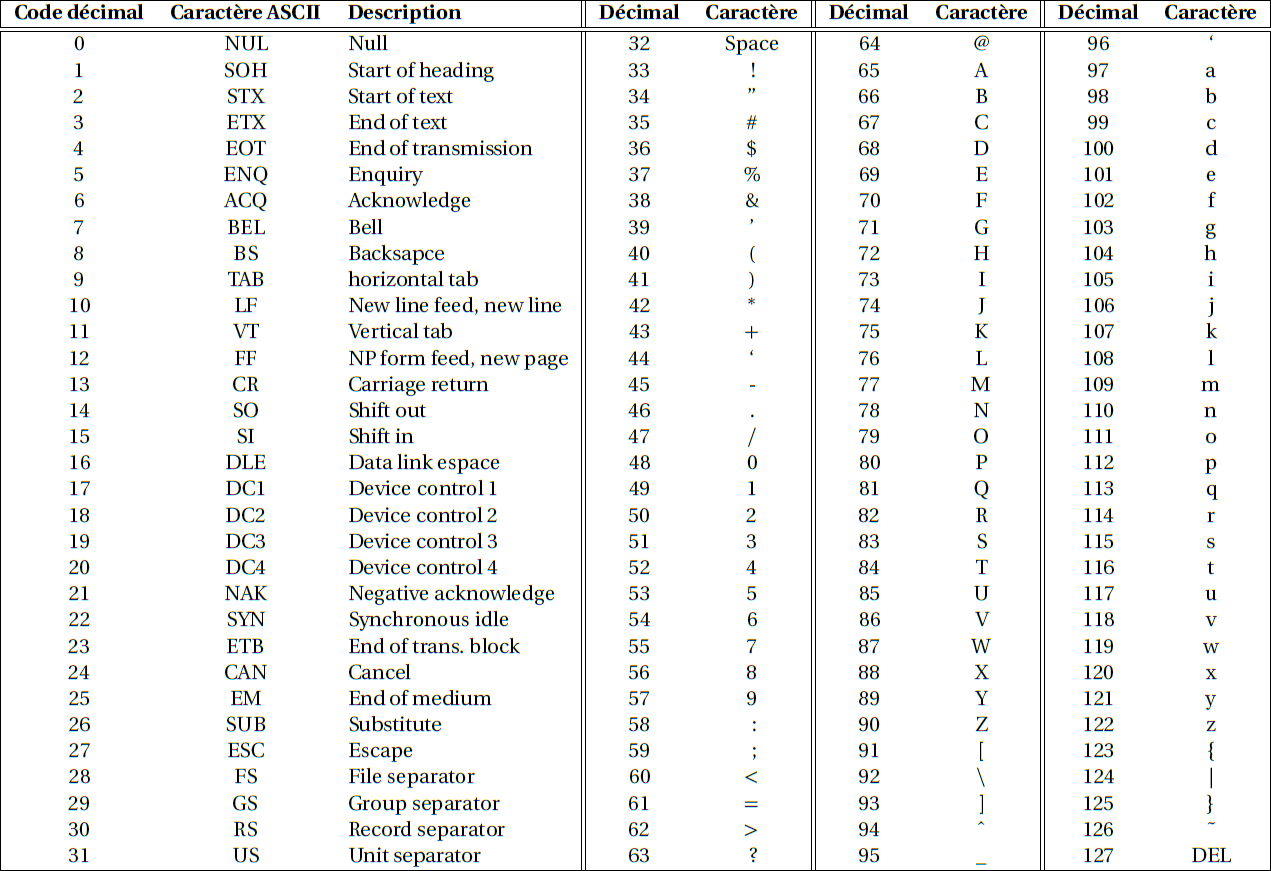
\includegraphics[width=\linewidth]{ascii}
\end{center}